\documentclass[border=4pt]{standalone}

\usepackage{pgfplots}
\pgfplotsset{compat=1.16}
\usepackage[T1]{fontenc}
\usepackage{lmodern}

\pgfplotsset{
  colormap={gray}{color(0cm)=(gray!0); color(1cm)=(gray!0!)}
}

\begin{document}

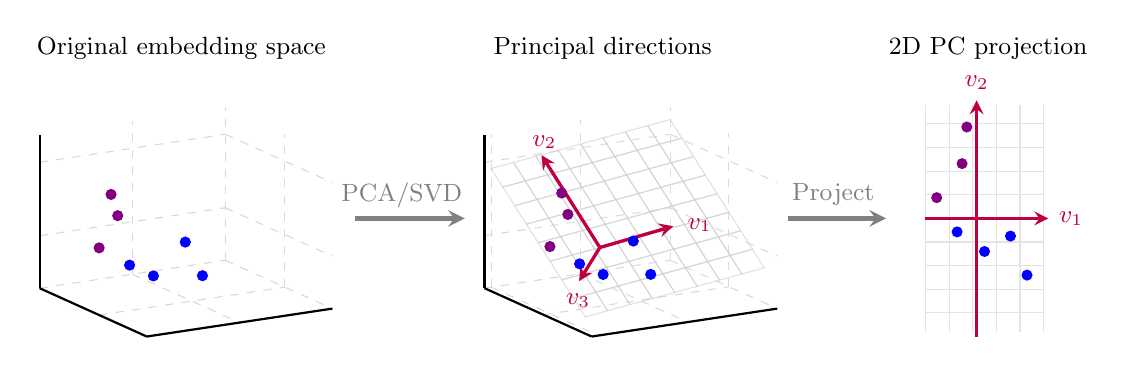
\begin{tikzpicture}[
    every node/.style={font=\small}
]

% ---------- shared point size ----------
\def\ptsize{1.8}

% =====================================================
% Panel 1: Original embedding space
% =====================================================
\begin{scope}[shift={(0,0)}]

\begin{axis}[
    view={60}{20},
    samples=9,
    grid=major,
    grid style={dashed,gray!30},
    width=5.3cm,
    height=4.5cm,
    axis lines*=left,
    axis line style=thick,
    ticks=none,
    domain=-0.5:0.3,
    domain y=0:1,
]

\addplot3[
    surf,
    domain=-0.5:0.3,
    domain y=0:1,
    fill opacity=0,
    draw opacity=0
] {-0.9*x+0.15*y};

\addplot3[only marks, mark=*, mark size=\ptsize, color=blue] coordinates
{(0.4,0.3,0.0) (0.3,0.1,0.0) (0.1,0.4,0.1) (0.1,0.1,0.0)};

\addplot3[only marks, mark=*, mark size=\ptsize, color=violet] coordinates
{(0.1,0,0.5) (0,0.1,0.3) (0,0,0.1)};

\end{axis}

\node[above] at (1.8,3.4) {Original embedding space};

\end{scope}

% Arrow 1
\draw[gray,-stealth,line width=1.6pt] (4,1.5) -- (5.4,1.5);
\node[gray,font=\small] at (4.6,1.8) {PCA/SVD};

% =====================================================
% Panel 2: Principal directions
% =====================================================
\begin{scope}[shift={(5.65,0)}]

\begin{axis}[
    view={60}{20},
    samples=9,
    grid=major,
    grid style={dashed,gray!30},
    width=5.3cm,
    height=4.5cm,
    axis lines*=left,
    axis line style=thick,
    ticks=none,
    domain=-0.5:0.3,
    domain y=0:1,
]

\addplot3[
    surf,
    domain=-0.5:0.3,
    domain y=0:1,
    fill opacity=0.13,
    draw opacity=0.58
] {-0.9*x+0.15*y};

\addplot3[-stealth,purple,line width=1.2pt] coordinates
{(0.12,0.2,0.1) (0.411,0.418,0.31)}
node[pos=1.05, right] {$v_1$};

\addplot3[-stealth,purple,line width=1.2pt] coordinates
{(0.12,0.2,0.1) (-0.3,0.15,0.586)}
node[pos=0.95, above] {$v_2$};

\addplot3[-stealth,purple,line width=1.2pt] coordinates
{(0.12,0.2,0.1) (0.304,-0.037,-0.019)}
node[pos=1.05, below] {$v_3$};

\addplot3[only marks, mark=*, mark size=\ptsize, color=blue] coordinates
{(0.4,0.3,0.0) (0.3,0.1,0.0) (0.1,0.4,0.1) (0.1,0.1,0.0)};

\addplot3[only marks, mark=*, mark size=\ptsize, color=violet] coordinates
{(0.1,0,0.5) (0,0.1,0.3) (0,0,0.1)};

\end{axis}

\node[above] at (1.5,3.4) {Principal directions};

\end{scope}

% Arrow 2
\draw[gray,-stealth,line width=1.6pt] (9.5,1.5) -- (10.75,1.5);
\node[gray,font=\small] at (10.08,1.8) {Project};

% % =====================================================
% Panel 3: 2D PC scores
% =====================================================
\begin{scope}[shift={(11.25,1.5)}]

% coordinate shrink factor
\def\s{0.3}

% grid
\draw[step={\s cm}, gray!22, thin]
    (0,{-4.8*\s}) grid ({5*\s},{4.8*\s});

% axes
\draw[-stealth,purple,line width=1.2pt]
    (0,0) -- ({5.2*\s},0) node[right] {$v_1$};

\draw[-stealth,purple,line width=1.2pt]
    (0.65,{-5.0*\s}) -- (0.65,{5.0*\s}) node[above] {$v_2$};

% projected points
\fill[blue] ({2.5*\s},{-1.4*\s}) circle[radius=2.0pt];
\fill[blue] ({4.3*\s},{-2.4*\s}) circle[radius=2.0pt];
\fill[blue] ({3.6*\s},{-0.748*\s}) circle[radius=2.0pt];
\fill[blue] ({1.34*\s},{-0.57*\s}) circle[radius=2.0pt];

\fill[violet] ({1.75*\s},{3.87*\s}) circle[radius=2.0pt];
\fill[violet] ({1.55*\s},{2.32*\s}) circle[radius=2.0pt];
\fill[violet] ({0.476*\s},{0.8788*\s}) circle[radius=2.0pt];

\node[font=\small] at ({2.65*\s},{5.55*\s + 0.5}) {2D PC projection};

\end{scope}

\end{tikzpicture}

\end{document}